\documentclass[12pt]{article}

\usepackage{sbc-template}
\usepackage[T1]{fontenc}
\usepackage[utf8]{inputenc}
\usepackage[brazilian]{babel}
\usepackage{graphicx,url}
\usepackage{tabularx}
\usepackage{float}
\usepackage{tikz}
\usetikzlibrary{positioning,arrows.meta}

\sloppy

\title{Identificação de Fibrose Renal por Visão Computacional em Imagens de Ultrassonografia}

\author{
  Jefferson S. dos Anjos\inst{1}, Amaro A. de Lima\inst{1},
  Gabriel M. Araújo\inst{1},\\ Jorge Luiz de C. Henriques Junior\inst{2},
  Norderval\inst{2}, Felipe da R. Henriques\inst{1}
}

\address{
  CEFET/RJ -- Rio de Janeiro -- RJ -- Brasil\\
  $^{2}$ HUPE -- UERJ -- Rio de Janeiro -- RJ -- Brasil\\
\vspace{-0.7cm}
\email{jefferson.anjos.1@aluno.cefet-rj.br,}\\
\vspace{-0.7cm}  \email{\{amaro.lima,gabriel.araujo,felipe.henriques\}@cefet-rj.br},\\
\vspace{-0.7cm}  \email{\{jorge.henriques,norderval.norderval\}@uerj.br}
}

\begin{document}

\maketitle

\begin{abstract}
This paper presents an ongoing research project aimed at analyzing ultrasound image patterns compatible with renal fibrosis using computer vision and deep learning. The study treats kidney segmentation as an intermediate step in a broader pipeline centered on renal region-of-interest analysis, intrarenal texture, echogenicity, and comparison with manually annotated reference organs such as the liver. The current version of the project already includes semantic segmentation models, pseudo-label based dataset expansion, quantitative intrarenal feature extraction, and a preliminary classifier. In the most recent comparative experiment, the best segmentation result was obtained by DeepLabV3 on the augmented dataset, with Dice of 0.8472. At the current stage, the results support the feasibility of extracting and analyzing potentially relevant imaging signs, but they do not yet constitute robust clinical identification of renal fibrosis because the labeled subset is still small and imbalanced.
\end{abstract}

\begin{resumo}
Este artigo apresenta um projeto de pesquisa em andamento voltado à análise de sinais imagéticos compatíveis com fibrose renal em imagens de ultrassonografia por meio de visão computacional e aprendizado profundo. O estudo trata a segmentação do rim como uma etapa intermediária de um pipeline mais amplo, centrado na análise da região de interesse renal, na textura intrarrenal, na ecogenicidade e na comparação com órgãos de referência anotados manualmente, como o fígado. A versão atual do projeto já inclui modelos de segmentação semântica, expansão de dataset por pseudo-rótulos, extração quantitativa de features intrarrenais e um classificador preliminar. No experimento comparativo mais recente, o melhor resultado de segmentação foi obtido pelo DeepLabV3 no dataset aumentado, com Dice de 0.8472. No estágio atual, os resultados sustentam a viabilidade de extrair e analisar sinais potencialmente relevantes, mas ainda não caracterizam identificação clínica robusta de fibrose renal, pois o subconjunto rotulado permanece pequeno e desbalanceado.
\end{resumo}

\section{Introdução}

A ultrassonografia renal é um exame amplamente utilizado por ser não invasivo, acessível e capaz de fornecer indícios relevantes sobre alterações estruturais do rim. Na prática clínica, a ecogenicidade do parênquima renal, em especial quando comparada à de órgãos próximos como o fígado, constitui um dos sinais mais observados na avaliação de doença renal crônica, conforme discutido por Manley e O'Neill (2001) e por Araújo et al. (2020). Apesar disso, a interpretação costuma depender fortemente da inspeção visual e da experiência do examinador.

Na literatura recente, a análise computacional de imagens renais tem avançado em duas frentes complementares. A primeira busca segmentar automaticamente o rim em imagens de ultrassonografia, como nos trabalhos de Ronneberger et al. (2015), Chen et al. (2022) e Xie et al. (2021). A segunda explora radiomics, textura e aprendizado de máquina para relacionar padrões intrarrenais com alterações fibróticas ou funcionais, como em Athavale et al. (2021), Chen et al. (2023) e Ge et al. (2023). Esse cenário sugere que a segmentação renal, embora necessária, não deve ser tratada como objetivo final, mas como base para uma análise quantitativa mais ampla da região renal.

Neste trabalho, a questão de pesquisa é a seguinte: em que medida a combinação entre segmentação do rim, extração de atributos intrarrenais e comparação com órgãos de referência pode apoiar a análise de sinais compatíveis com fibrose renal em ultrassom? Parte-se da hipótese de que a análise conjunta de ecogenicidade, heterogeneidade intrarrenal, concentração de pontos brilhantes e máscara interna candidata das pirâmides renais pode produzir descrições quantitativas úteis para separar rins potencialmente saudáveis de rins com suspeita de alteração, em linha com as evidências apresentadas por Manley e O'Neill (2001), Chavhan et al. (2008), Chen et al. (2023) e Ge et al. (2023).

O objetivo deste artigo é apresentar a formulação atual do problema, a solução metodológica em desenvolvimento e os resultados experimentais já obtidos. As principais contribuições do estudo são: a consolidação de um benchmark interno entre U-Net, UNet++, DeepLabV3 e SegFormer; a avaliação do impacto de uma variante de dataset aumentada por pseudo-rótulos; a extração sistemática de features intrarrenais sobre a região segmentada; e a implementação de um classificador experimental baseado em Random Forest para avaliação preliminar da capacidade do pipeline de analisar sinais compatíveis com alteração renal.

O restante do artigo está organizado da seguinte forma. A Seção 2 apresenta a fundamentação teórica. A Seção 3 discute os trabalhos relacionados. A Seção 4 descreve a metodologia proposta. A Seção 5 apresenta a avaliação experimental, incluindo configuração, métricas, resultados e limitações. Por fim, a Seção 6 apresenta as conclusões e os próximos passos do estudo.

\section{Fundamentação Teórica}

\subsection{Ecogenicidade Renal e Comparação com Órgãos de Referência}

A avaliação da ecogenicidade renal é um dos elementos clássicos da ultrassonografia em nefrologia. Manley e O'Neill (2001) propuseram uma quantificação objetiva da ecogenicidade cortical renal com base na razão entre a intensidade do córtex renal e a do fígado. Nesse estudo, os autores mostraram que a ecogenicidade pode ser expressa como uma razão quantitativa entre regiões de interesse, reduzindo a dependência exclusiva da inspeção visual.

Trabalhos posteriores reforçaram a relevância clínica dessa comparação. Araújo et al. (2020) mostraram que parâmetros ultrassonográficos ponderados pela ecogenicidade cortical apresentaram melhor capacidade de predizer alterações histológicas crônicas e pior função renal do que medidas brutas isoladas. Em particular, o estudo sugere que a ecogenicidade cortical relativa ao fígado pode acrescentar valor à interpretação clínica da imagem.

\subsection{Textura, Radiomics e Fibrose Renal}

A literatura recente passou a explorar radiomics e aprendizado de máquina para quantificar padrões intrarrenais em ultrassom. Chen et al. (2023) desenvolveram um modelo de radiomics com imagens ultrassonográficas e características clínicas para avaliar a gravidade da fibrose renal em pacientes com doença renal crônica. Ge et al. (2023) propuseram um modelo multimodal baseado em ultrassom e radiomics para detecção de fibrose, mostrando que a combinação de informações quantitativas pode superar abordagens baseadas em indicadores clínicos isolados.

Esses trabalhos indicam que a análise da imagem não precisa se limitar ao contorno do rim. Atributos como intensidade média, heterogeneidade local, distribuição de brilho e padrões de textura podem carregar informação diagnóstica relevante sobre o estado do parênquima renal, como apontado por Chen et al. (2023) e Ge et al. (2023).
Em particular, descritores derivados de matrizes de coocorrência de níveis de cinza continuam sendo uma base clássica para quantificação de textura, desde a formulação proposta por Haralick et al.~\cite{Haralick1973}.

\subsection{Pirâmides Renais como Alvo Anatômico}

Além da análise global do parênquima, a literatura também indica que alterações nas pirâmides renais merecem atenção. Chavhan et al. (2008) relataram correlação entre mudanças de ecogenicidade das pirâmides renais e pior função renal diferencial em um contexto pediátrico. Embora o cenário clínico seja específico, o trabalho ajuda a justificar o uso das pirâmides como alvo anatômico de interesse em sistemas computacionais de apoio à decisão.

\subsection{Arquiteturas de Segmentação Utilizadas}

Como etapa inicial do projeto, foram avaliadas arquiteturas consolidadas de segmentação semântica aplicadas à imagem médica. A U-Net, proposta por Ronneberger et al. (2015), tornou-se uma referência por combinar caminho de contração e expansão com conexões de atalho, preservando detalhes espaciais importantes em tarefas biomédicas. A UNet++, apresentada por Zhou et al. (2018), estende essa ideia com conexões aninhadas entre blocos intermediários, buscando reduzir a lacuna semântica entre codificador e decodificador.

Também foi considerada a arquitetura DeepLabV3, em sua variante encoder-decoder com convoluções separáveis atrous, descrita por Chen et al. (2018), por sua capacidade de capturar contexto multi-escala. Por fim, foi incluído o SegFormer, proposto por Xie et al. (2021), uma arquitetura baseada em transformers para segmentação semântica, com codificador hierárquico e decodificador leve. A escolha desses modelos se justifica por representarem estratégias complementares no problema de segmentação renal.

\section{Trabalhos Relacionados}

Uma linha importante de pesquisa é a segmentação automática do rim em imagens de ultrassonografia. Chen et al. (2022) apresentaram uma arquitetura convolucional multiescala com supervisão profunda para segmentação renal, obtendo desempenho elevado em métricas como Dice, Jaccard, precisão e recall. Esses trabalhos são diretamente relevantes porque estabelecem a segmentação do rim como etapa base para o isolamento anatômico da região de interesse renal.

Outra referência central é o trabalho de Athavale et al. (2021), que propôs um pipeline composto por pré-processamento, segmentação renal com U-Net, extração de atributos com VGG19 e classificação com extreme gradient boosting para quantificar interstitial fibrosis and tubular atrophy (IFTA) a partir de imagens de ultrassonografia. Esse estudo é especialmente importante porque demonstra que a segmentação do rim pode ser tratada como uma etapa intermediária de um sistema mais amplo orientado à caracterização patológica.

Em comparação com esses trabalhos, o presente estudo concentra-se em um pipeline híbrido e incremental. Em vez de propor apenas um novo segmentador, o trabalho compara diferentes famílias de modelos de segmentação, investiga o efeito da expansão do dataset por pseudo-rótulos e explora a extração de features intrarrenais combinada à comparação rim-fígado. Assim, a principal lacuna abordada aqui não é apenas “onde está o rim?”, mas também “como transformar a região segmentada em evidência quantitativa útil para análise de fibrose?”.

\section{Metodologia Proposta}

\subsection{Visão Geral do Pipeline}

Com base no estado atual da literatura e na organização do projeto, propõe-se o seguinte pipeline metodológico:

\begin{enumerate}
\item pré-processamento da imagem, incluindo normalização, redimensionamento e preparo da entrada para os modelos de segmentação;
\item segmentação automática do rim com arquiteturas já avaliadas no projeto;
\item geração da região de interesse renal a partir da máscara segmentada;
\item extração de atributos intrarrenais, como intensidade média, desvio padrão, percentis, textura por matrizes de coocorrência e proporção de pontos brilhantes;
\item obtenção de uma máscara interna candidata das pirâmides renais por heurísticas baseadas em intensidade e morfologia;
\item comparação entre a intensidade média do rim e a intensidade média de uma ROI manual do fígado, quando essa estrutura estiver visível no exame;
\item classificação experimental preliminar do rim em categorias binárias, a partir das features extraídas.
\end{enumerate}

Esse desenho segue a lógica dos trabalhos de Athavale et al. (2021), Chen et al. (2023) e Ge et al. (2023), ao mesmo tempo em que incorpora a comparação rim-fígado inspirada por Manley e O'Neill (2001) e pelo uso clínico de ecogenicidade relativa discutido por Araújo et al. (2020).

A Figura~\ref{fig:tikz_pipeline} resume visualmente o encadeamento principal do método proposto, desde a entrada da imagem até a etapa de análise intrarrenal.

\begin{figure}[H]
\centering
\begin{tikzpicture}[
    node distance=0.55cm and 0.8cm,
    >=Latex,
    every node/.style={font=\small, align=center},
    block/.style={
        draw,
        rounded corners=2pt,
        minimum width=3.2cm,
        minimum height=1.0cm,
        fill=gray!8
    }
]
\node[block] (input) {Imagens de\\ultrassonografia};
\node[block, right=of input] (prep) {Pre-processamento\\e padronização};
\node[block, right=of prep] (seg) {Segmentação\\renal};
\node[block, right=of seg] (mask) {Máscara binária\\do rim};
\node[block, below=of seg] (roi) {ROI renal e\\features intrarrenais};
\node[block, left=of roi] (analysis) {Análise de sinais\\compatíveis com fibrose};

\draw[->, thick] (input) -- (prep);
\draw[->, thick] (prep) -- (seg);
\draw[->, thick] (seg) -- (mask);
\draw[->, thick] (mask) -- (roi);
\draw[->, thick] (roi) -- (analysis);
\end{tikzpicture}
\caption{Diagrama resumido do pipeline metodológico proposto. A segmentação renal atua como etapa intermediária entre o pré-processamento das imagens e a análise quantitativa de sinais compatíveis com fibrose.}
\label{fig:tikz_pipeline}
\end{figure}

Esse diagrama resume a hipótese operacional do trabalho: a segmentação não é tratada como fim em si mesma, mas como suporte para uma etapa posterior de análise quantitativa da região renal.

A Figura 1 ilustra qualitativamente um caso em que a comparação rim-referência é incorporada ao pipeline. Quando o rim apresenta brilho relativamente aumentado em comparação com o órgão adjacente, a razão de intensidades passa a funcionar como um indício quantitativo complementar à análise visual.

\begin{figure}[H]
\centering
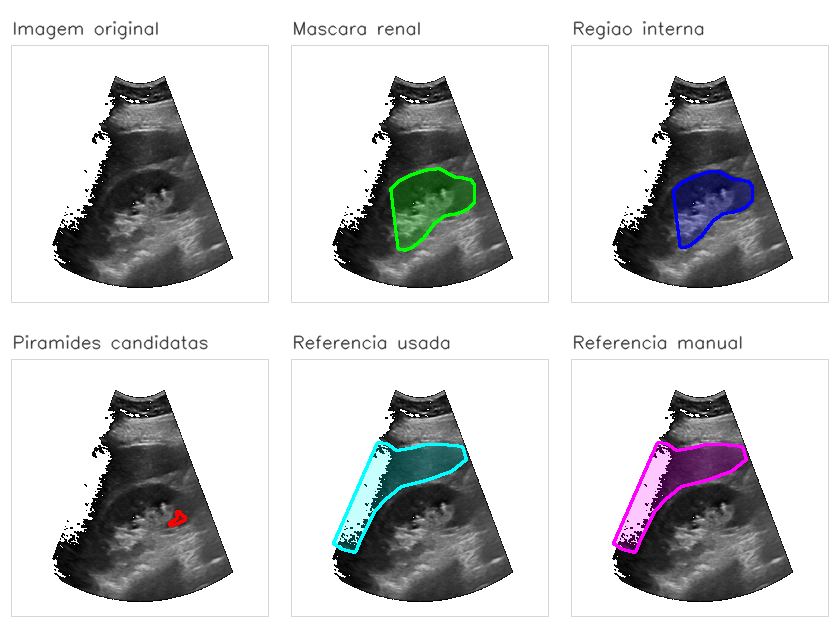
\includegraphics[width=0.74\textwidth]{figures/example_reference_high_ratio_1.png}
\caption{Exemplo qualitativo do pipeline de análise com órgão de referência. O painel apresenta a imagem original, a máscara renal, a região intrarrenal analisada, as pirâmides renais candidatas e as regiões de referência automática e manual empregadas na comparação de ecogenicidade.}
\label{fig:reference_example}
\end{figure}

O exemplo mostra que, uma vez obtida a máscara renal, o pipeline já consegue estruturar a região de interesse e produzir comparações quantitativas potencialmente úteis para a análise de ecogenicidade relativa.

\subsection{Base de Dados e Variantes Experimentais}

O projeto passou por uma etapa específica de engenharia de dados para ampliar a base usada na segmentação renal. O acervo inicial estava organizado em treino, validação e teste, totalizando 513 pares imagem-máscara em \texttt{dataset/}, distribuídos em 360 imagens de treino, 51 de validação e 102 de teste. Esse acervo deriva da base pública Open Kidney Ultrasound Data Set, descrita por Singla et al.~\cite{Singla2023KidneyUS}. Em uma primeira expansão local, foi criado um fluxo de pseudo-labeling sobre o material bruto, em linha com a estratégia clássica de geração automática de rótulos proposta por Lee~\cite{Lee2013PseudoLabel}, resultando em uma versão expandida em \texttt{dataset\_augmented/}.

Na etapa mais recente, a busca por dados externos considerou repositórios públicos e índices de ultrassonografia, incluindo o Open Kidney Ultrasound Data Set~\cite{Singla2023KidneyUS}, o índice NIDUS/RadOSS~\cite{NIDUS2026}, o Clinical Ultrasound Image Repository mantido pela comunidade MONAI/NVIDIA~\cite{MONAIClinicalUltrasound}, o dataset abdominal da Mississippi State University~\cite{Karim2025AbdominalUS}, o TRUSTED~\cite{Ndzimbong2025TRUSTED}, coleções Kaggle de ultrassom renal~\cite{KaurKaggleKidneyStone,BnouiriKaggleRenalData} e o repositório CGPxy~\cite{CGPxyUltrasoundDataset}. Como o MONAI é amplo e heterogêneo, contendo estudos abdominais, cardíacos e obstétricos, a estratégia adotada foi baixar os estudos renais em partes, converter apenas quadros DICOM úteis para PNG, rejeitar imagens RGB/coloridas ou com sobreposições, manter somente ultrassom B-mode em escala de cinza e apagar os arquivos brutos após validação dos manifestos.

O resultado dessa engenharia foi consolidado em \texttt{dataset\_geral/}. A montagem atual contém 5.994 imagens únicas; dessas, 3.962 possuem máscaras aceitas, sendo 1.001 máscaras já existentes e 2.961 pseudo-máscaras geradas automaticamente com limiar operacional de confiança de 0.90 e filtros de área, componentes conectados e pixels de primeiro plano. As 2.032 imagens restantes permanecem no manifesto como casos sem máscara aceita, não sendo usadas no treinamento supervisionado até revisão ou nova geração de máscaras.

Para o novo ciclo de treinamento, o estudo passa a usar as 3.962 imagens com máscara aceita em \texttt{dataset\_geral}. O protocolo separa 30\% do conjunto como teste final fixo, totalizando 1.188 imagens, e reserva os 70\% restantes para treino e seleção de modelo, totalizando 2.774 imagens. Dentro desses 70\%, foi criada uma validação cruzada em 5 folds: em cada rodada, aproximadamente 2.215 a 2.221 imagens são usadas para treino e 553 a 559 imagens para validação, mantendo o mesmo conjunto de teste final para a avaliação externa do modelo treinado. Esse desenho evita escolher hiperparâmetros diretamente sobre o teste final e permite estimar a estabilidade da segmentação antes de definir o modelo a ser usado nas etapas posteriores de análise renal.

\subsection{Modelos de Segmentação, Features e Classificação}

O estudo avalia quatro famílias de segmentadores: U-Net, UNet++, DeepLabV3 e SegFormer. Para cada família, são consideradas variantes baseline e variantes com ajustes de capacidade ou hiperparâmetros, sempre com avaliação no conjunto de teste correspondente à versão do acervo utilizada. O objetivo não é apenas identificar o melhor modelo absoluto, mas também verificar a robustez das famílias de segmentação sob diferentes condições de treinamento.

Após a segmentação do rim, o pipeline extrai features intrarrenais quantitativas da região de interesse renal. Entre essas features estão intensidade média, medidas de dispersão, percentis, atributos de textura baseados em matrizes de coocorrência de níveis de cinza~\cite{Haralick1973} e proporção de pixels brilhantes. Quando existe uma ROI manual de fígado, o sistema também calcula razões rim-fígado e interior-do-rim-fígado. Na etapa de classificação, é usado um classificador Random Forest com imputação por mediana~\cite{Breiman2001}, servindo como prova de conceito para a utilidade das features extraídas.

\section{Avaliação Experimental}

\subsection{Desenho Experimental}

A avaliação experimental tem dois objetivos. O primeiro é verificar se a etapa de segmentação renal é suficientemente robusta para sustentar a análise subsequente da região de interesse. O segundo é investigar se as features intrarrenais extraídas da região segmentada já carregam sinal útil para uma classificação preliminar de rins com e sem suspeita de alteração.

No experimento de segmentação, os resultados obtidos anteriormente com \texttt{dataset\_augmented/} são mantidos como linha de base histórica do projeto. A partir da nova engenharia de dados, o benchmark principal passa a ser orientado por \texttt{dataset\_geral/}, com separação 70/30 e validação cruzada em 5 folds dentro dos 70\% de treino/desenvolvimento. Esse novo protocolo foi estruturado para treinar um segmentador mais robusto com maior diversidade de imagens e com avaliação final preservada em um holdout independente.

No experimento de classificação, a avaliação é necessariamente mais restrita. O subconjunto rotulado disponível contém apenas 50 imagens, com forte desbalanceamento entre classes. Desse total, 44 amostras foram usadas em treino/validação e 6 no subconjunto de teste. Por essa razão, o classificador deve ser interpretado como estudo exploratório de viabilidade e não como modelo validado clinicamente.

\subsection{Métricas de Avaliação}

As métricas adotadas na segmentação têm papéis complementares. O coeficiente Dice mede a sobreposição entre a máscara predita e a máscara de referência, sendo amplamente usado em segmentação médica. A IoU (\textit{Intersection over Union}) também quantifica sobreposição, mas de forma mais rígida. A precisão (\textit{Precision}) indica a proporção de pixels preditos como rim que realmente pertencem ao rim, enquanto o recall mede a capacidade do modelo de recuperar todos os pixels da estrutura-alvo. O F1-score sintetiza precisão e recall em uma média harmônica. A distância de Hausdorff avalia discrepâncias geométricas mais severas entre contornos, sendo útil para detectar erros localizados de borda. Por fim, FPS (\textit{frames per second}) expressa o custo computacional da inferência e indica a velocidade de processamento do modelo. A escolha desse conjunto segue a recomendação de combinar métricas de sobreposição e de contorno na avaliação de segmentação médica, como discutido por Taha e Hanbury~\cite{Taha2015Metrics}.

Na classificação, a acurácia representa a proporção total de imagens corretamente classificadas. A precisão indica, entre os casos preditos como doentes, quantos realmente pertencem a essa classe. O recall mede a capacidade do modelo de recuperar os casos alterados presentes no conjunto avaliado. O F1-score sintetiza o equilíbrio entre precisão e recall, enquanto a ROC-AUC mede a capacidade do classificador de separar as classes ao longo de diferentes limiares de decisão.

\subsection{Resultados de Segmentação}

A Tabela~\ref{tab:deeplab_dataset_geral_cv} apresenta o novo resultado de segmentação obtido com DeepLabV3 ResNet50 sobre o \texttt{dataset\_geral}. O treinamento utilizou validação cruzada em 5 folds dentro dos 70\% de desenvolvimento e manteve 30\% da base supervisionada como teste final fixo. O desempenho médio no teste foi de Dice 0.9366 e IoU 0.8839, com melhor fold atingindo Dice 0.9420 e IoU 0.8904. Esse resultado passa a ser a principal referência experimental do projeto para segmentação renal.

\begin{table}[H]
\centering
\caption{Resultados do DeepLabV3 ResNet50 no \texttt{dataset\_geral} com validação cruzada em 5 folds e teste final fixo de 30\%.}
\label{tab:deeplab_dataset_geral_cv}
\begin{tabular}{lccccc}
\hline
\textbf{Fold} & \textbf{Época} & \textbf{Limiar} & \textbf{Dice Val.} & \textbf{Dice Teste} & \textbf{IoU Teste} \\
\hline
1 & 25 & 0.50 & 0.9298 & 0.9263 & 0.8782 \\
2 & 16 & 0.50 & 0.9358 & 0.9371 & 0.8817 \\
3 & 19 & 0.55 & 0.9401 & 0.9391 & 0.8851 \\
4 & 18 & 0.50 & 0.9467 & \textbf{0.9420} & \textbf{0.8904} \\
5 & 17 & 0.35 & 0.9400 & 0.9385 & 0.8841 \\
\hline
\textbf{Média} & -- & -- & \textbf{0.9385} & \textbf{0.9366} & \textbf{0.8839} \\
\hline
\end{tabular}
\end{table}

A Tabela~\ref{tab:benchmark_segmentacao} mantém a linha de base anterior por família de modelo na versão expandida antiga do acervo principal, representada por \texttt{dataset\_augmented/}. O objetivo dessa comparação histórica é mostrar o salto obtido após a engenharia do \texttt{dataset\_geral}, sem misturar protocolos experimentais distintos.

\begin{table}[H]
\centering
\caption{Melhores resultados de segmentação renal por família de modelo na versão expandida do acervo principal (\texttt{dataset\_augmented/}).}
\label{tab:benchmark_segmentacao}
\begin{tabular}{lccccccc}
\hline
\textbf{Modelo} & \textbf{Dice} & \textbf{IoU} & \textbf{Precision} & \textbf{Recall} & \textbf{F1} & \textbf{Hausdorff} & \textbf{FPS} \\
\hline
DeepLabV3 & 0.8472 & 0.7732 & 0.8426 & 0.8718 & 0.8472 & 18.02 & 28.98 \\
SegFormer & 0.8372 & 0.7700 & 0.8294 & 0.8782 & 0.8372 & 17.46 & 35.66 \\
U-Net & 0.8119 & 0.7309 & 0.8039 & 0.8545 & 0.8119 & 23.60 & 26.43 \\
UNet++ & 0.7924 & 0.6958 & 0.8189 & 0.7968 & 0.7924 & 31.90 & 20.88 \\
\hline
\end{tabular}
\end{table}

Na linha de base anterior, o melhor desempenho global havia sido obtido pelo DeepLabV3 treinado na versão expandida do acervo principal, \texttt{dataset\_augmented/}, com Dice de 0.8472. O SegFormer permaneceu muito competitivo, com Dice de 0.8372, menor Hausdorff do que o DeepLab e melhor relação entre qualidade e velocidade de inferência entre os modelos de maior desempenho. Naquele conjunto avaliado, a U-Net baseline e a UNet++ baseline seguiram como alternativas competitivas, embora abaixo das variantes de DeepLab e SegFormer no topo do benchmark.

Em verificações internas realizadas durante o desenvolvimento, a expansão por pseudo-rótulos mostrou tendência favorável para a maior parte das variantes baseline, o que motivou inicialmente a adoção de \texttt{dataset\_augmented/}. A nova montagem \texttt{dataset\_geral/} amplia essa lógica ao incorporar fontes externas curadas e pseudo-máscaras filtradas, elevando o desempenho do DeepLabV3 em relação ao benchmark anterior.

Como referência externa, o projeto passou a comparar seus resultados com artefatos do \texttt{kidneyUS}, a partir de métricas de validação associadas a pesos \texttt{nnUNet}. Além dessa comparação, o ambiente experimental deste trabalho agora suporta inferência nativa com a mesma família de modelos usada no projeto de referência, isto é, \texttt{nnUNet} em modo \texttt{2d} para a tarefa \texttt{Task001\_KidneyCapsule}. Considerando essa tarefa, que é a mais próxima da segmentação binária externa do rim usada neste estudo, o melhor resultado local atual ficou entre 2.6 e 3.8 pontos de Dice abaixo das referências externas, que variaram entre 0.8729 e 0.8852.

Em uma reprodução nativa preliminar com esse mesmo \texttt{nnUNet}, executada sobre as 102 imagens do split de teste local e usando as imagens originais em maior resolução, obteve-se Dice médio de 0.6821, IoU de 0.6307, precisão de 0.7404, recall de 0.6697 e Hausdorff médio de 18.4468. Esse resultado ficou abaixo dos melhores modelos treinados diretamente neste repositório, sugerindo que a transferência direta do modelo externo para o protocolo local não é suficiente para superar o ajuste específico obtido com os dados e máscaras usados neste trabalho. Assim, a comparação com o \texttt{kidneyUS} é útil como contextualização do estado da arte e da linha metodológica adotada, mas a Tabela 2 ainda reflete apenas o benchmark local consolidado.

A Tabela 2 consolida todos os resultados quantitativos das execuções de segmentação consideradas no benchmark local sobre o dataset final do trabalho, isto é, a versão expandida do acervo principal. Essa visão completa é importante porque mostra que o melhor desempenho global não depende apenas da família do modelo, mas também da configuração de treino adotada dentro de uma mesma base final.

\begin{table}[H]
\centering
\caption{Resultados completos das execuções de segmentação avaliadas no dataset final expandido do trabalho.}
\label{tab:todos_modelos_segmentacao}
\scriptsize
\begin{tabular}{lccccc}
\hline
\textbf{Modelo / Configuração} & \textbf{Dice} & \textbf{IoU} & \textbf{Precision} & \textbf{Recall} & \textbf{FPS} \\
\hline
DeepLab R50 baseline & \textbf{0.8472} & \textbf{0.7732} & \textbf{0.8426} & 0.8718 & 28.98 \\
DeepLab R101 capacity & 0.8376 & 0.7700 & 0.8419 & 0.8638 & 23.68 \\
SegFormer B2 capacity & 0.8372 & 0.7700 & 0.8294 & \textbf{0.8782} & 35.66 \\
SegFormer B0 baseline & 0.8167 & 0.7353 & 0.8140 & 0.8410 & \textbf{47.91} \\
U-Net baseline & 0.8119 & 0.7309 & 0.8039 & 0.8545 & 26.43 \\
U-Net capacity & 0.8046 & 0.7181 & 0.7758 & 0.8734 & 17.69 \\
U-Net 320 px & 0.6183 & 0.5289 & 0.8020 & 0.5524 & 10.99 \\
UNet++ baseline & 0.7924 & 0.6958 & 0.8189 & 0.7968 & 20.88 \\
UNet++ capacity & 0.6974 & 0.5731 & 0.6909 & 0.7649 & 12.03 \\
\hline
\end{tabular}
\normalsize
\end{table}

Na Tabela 2, os valores em negrito destacam os melhores resultados por métrica entre todas as execuções listadas para a base final. Observa-se que o melhor equilíbrio global continua com o DeepLab R50 baseline, que lidera em Dice, IoU e precisão e, por isso, permanece como a configuração mais promissora para segmentação renal no estado atual do projeto. O maior recall foi obtido pelo SegFormer B2 capacity, indicando que essa família segue muito competitiva quando o objetivo é recuperar a maior extensão possível do rim.

Também é relevante notar o trade-off entre qualidade e custo computacional. O SegFormer B0 baseline apresentou o maior FPS da tabela, mostrando que há opções mais rápidas com perda moderada de qualidade. Em contraste, as variantes de alta resolução da U-Net ficaram entre as piores em Dice e IoU, indicando que aumentar a resolução de entrada, neste cenário, não trouxe ganho proporcional. No conjunto geral, as arquiteturas DeepLab e SegFormer concentraram o topo do benchmark, enquanto variantes baseline bem ajustadas superaram várias configurações mais pesadas.

\subsection{Influência da Qualidade da Imagem}

Além das métricas agregadas, a inspeção qualitativa indica que a qualidade da imagem exerce papel decisivo na dificuldade da segmentação. Em exames mais favoráveis, com contorno renal relativamente completo, contraste mais estável e menos artefatos, tanto o projeto concorrente quanto o modelo local conseguem recuperar a estrutura global do rim. Ainda assim, a Figura~\ref{fig:quality_good} mostra que, em um caso de boa visualização, o DeepLab local produziu contorno mais aderente à máscara de referência do que o \texttt{kidneyUS}, com Dice de 0.9660 contra 0.7789 nessa amostra.

\begin{figure}[H]
\centering
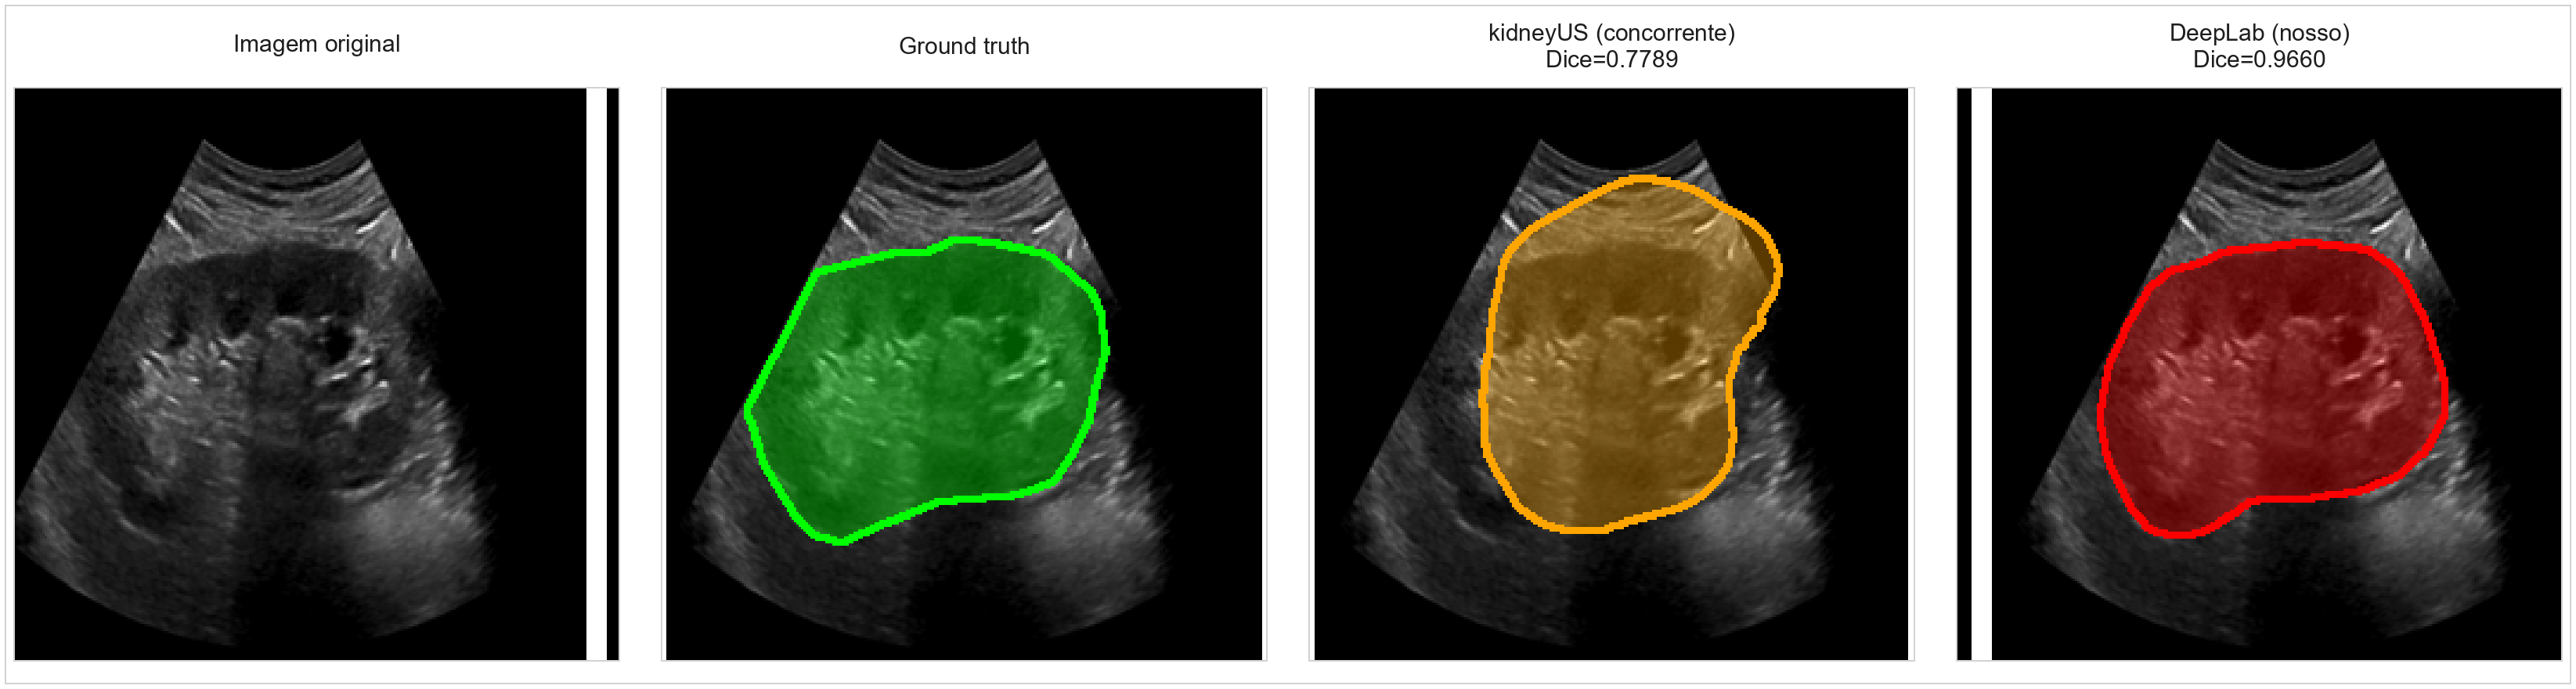
\includegraphics[width=0.92\textwidth]{figures/quality_good_comparison.png}
\caption{Caso qualitativo favorável. Da esquerda para a direita, são mostradas a imagem original, a máscara de referência, a segmentação produzida pelo \texttt{kidneyUS} e a segmentação produzida pelo DeepLab local. Nesse exemplo, o contorno local apresenta maior aderência à referência anatômica.}
\label{fig:quality_good}
\end{figure}

Nesse cenário, a boa definição do contorno renal favorece ambos os métodos, mas a predição local preserva melhor a geometria global da estrutura segmentada.

Em contrapartida, quando a imagem apresenta contraste reduzido, textura mais ruidosa ou menor nitidez anatômica, a tarefa se torna substancialmente mais difícil. A Figura~\ref{fig:quality_bad} ilustra um caso de pior qualidade visual em que o \texttt{kidneyUS} falhou completamente nessa amostra, com Dice igual a 0.0, enquanto o DeepLab local ainda preservou uma segmentação parcialmente utilizável, com Dice de 0.8172. Esse comportamento reforça que parte da variabilidade observada nos resultados não decorre apenas da arquitetura, mas também da legibilidade do rim no ultrassom.

\begin{figure}[H]
\centering
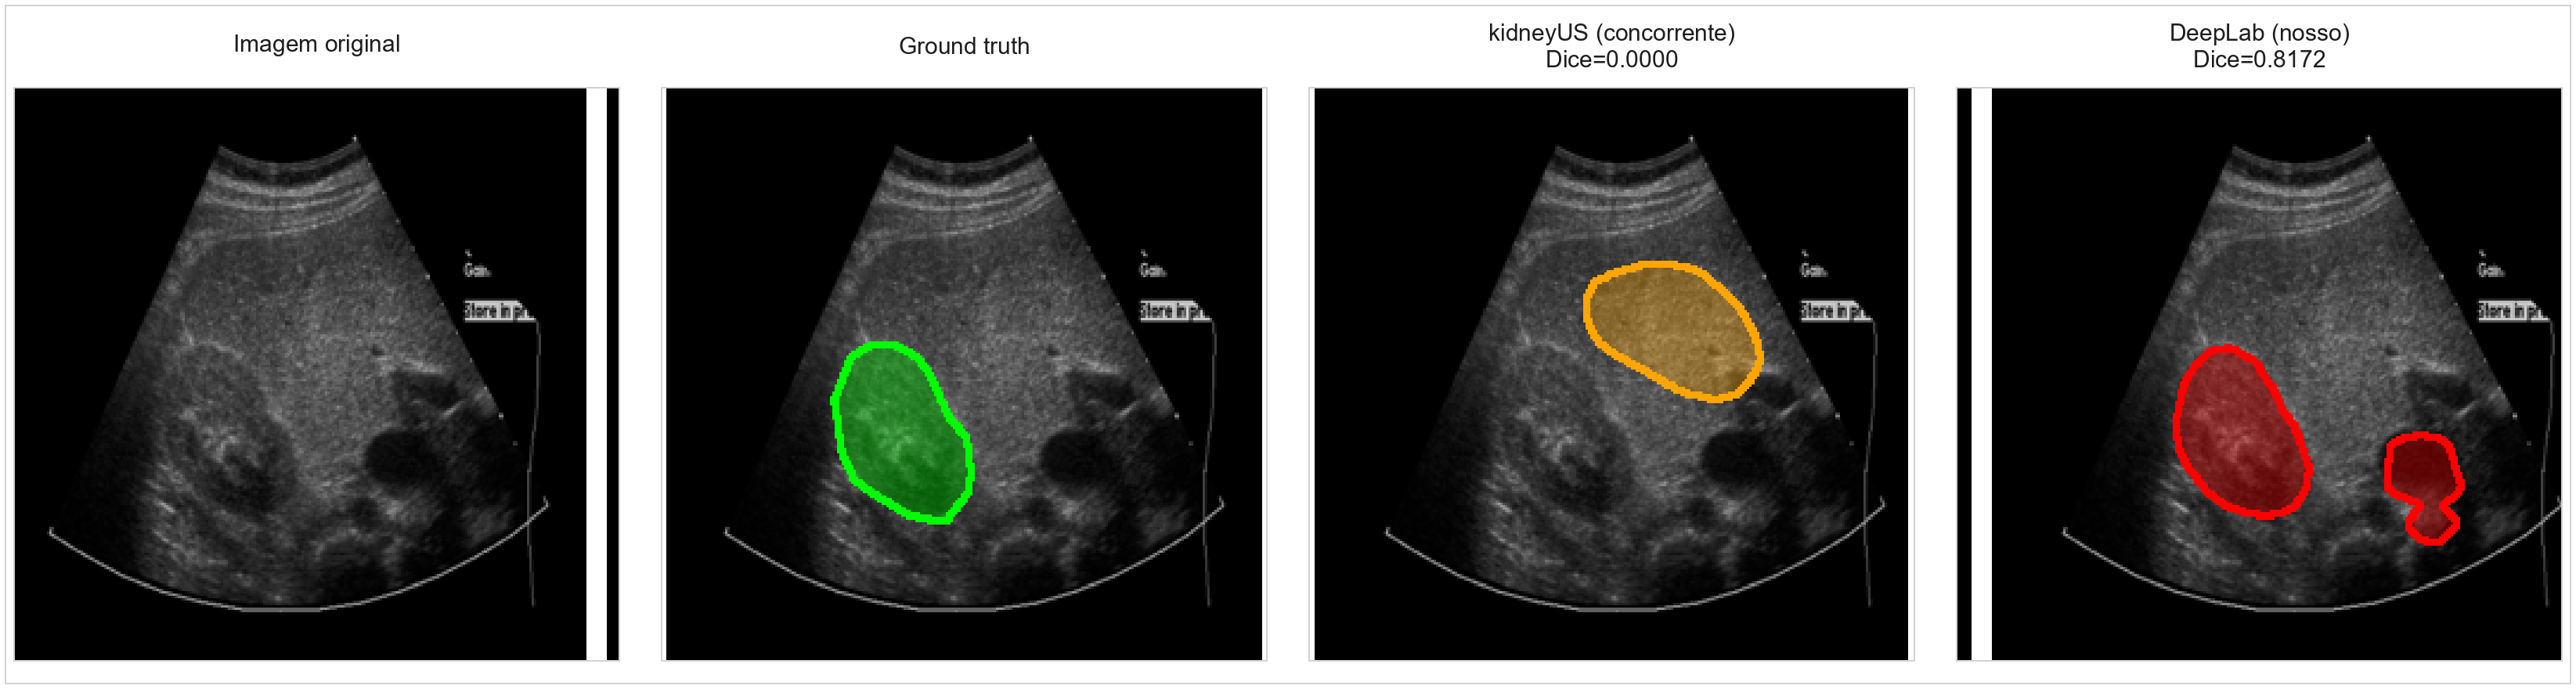
\includegraphics[width=0.92\textwidth]{figures/quality_bad_comparison.png}
\caption{Caso qualitativo desafiador. Da esquerda para a direita, observam-se a imagem original, a máscara de referência, a predição do \texttt{kidneyUS} e a predição do DeepLab local. Em condição de menor legibilidade anatômica, o método concorrente desloca a segmentação para uma região incorreta, enquanto o modelo local preserva parcialmente o contorno renal.}
\label{fig:quality_bad}
\end{figure}

Esse contraste entre os dois casos qualitativos reforça que a robustez da segmentação depende não apenas da arquitetura empregada, mas também da qualidade visual e da completude anatômica do exame.

\subsection{Resultados de Classificação}

As Figuras~\ref{fig:diseased_example} e~\ref{fig:healthy_example} apresentam dois exemplos qualitativos extraídos diretamente do pipeline: um caso com predição positiva e um caso com predição negativa do classificador experimental.

\begin{figure}[H]
\centering
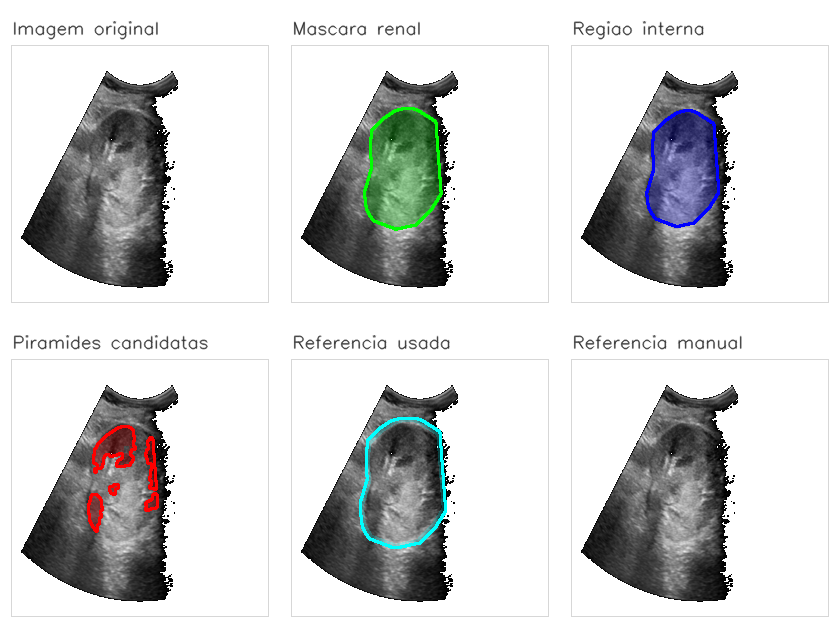
\includegraphics[width=0.74\textwidth]{figures/example_predicted_diseased_1.png}
\caption{Exemplo do subconjunto rotulado com predição positiva do classificador experimental, correspondente à classe com suspeita de alteração.}
\label{fig:diseased_example}
\end{figure}

\begin{figure}[H]
\centering
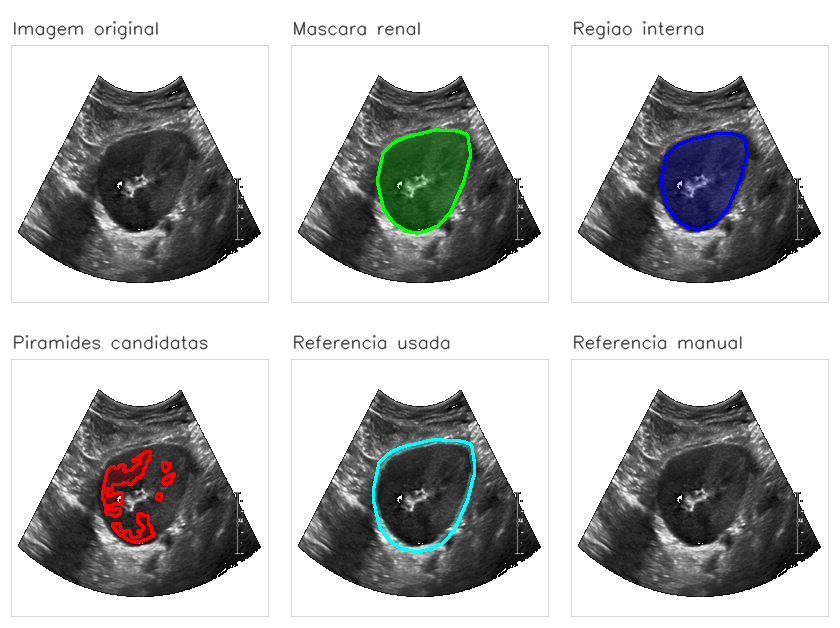
\includegraphics[width=0.74\textwidth]{figures/example_predicted_healthy_1.png}
\caption{Exemplo do subconjunto rotulado com predição negativa do classificador experimental, correspondente à classe sem suspeita de alteração.}
\label{fig:healthy_example}
\end{figure}

Em conjunto, os dois exemplos qualitativos da classificação servem apenas como ilustração do comportamento do pipeline e não substituem a interpretação quantitativa apresentada na Tabela 3.

A Tabela 3 resume o desempenho do classificador experimental no subconjunto de teste rotulado. Diferentemente da etapa de segmentação, que passou a ser discutida em alinhamento metodológico com o \texttt{kidneyUS}, essa classificação não faz parte do pipeline original do projeto de referência. Trata-se de uma etapa exploratória própria deste trabalho, construída a partir das features intrarrenais extraídas após a segmentação, e implementada com um classificador \textit{Random Forest}.

\begin{table}[H]
\centering
\caption{Resultados do classificador experimental no subconjunto de teste rotulado.}
\label{tab:benchmark_classificacao}
\begin{tabular}{lccccc}
\hline
\textbf{Modelo} & \textbf{Accuracy} & \textbf{Precision} & \textbf{Recall} & \textbf{F1} & \textbf{ROC-AUC} \\
\hline
Random Forest & 0.8333 & 1.0000 & 0.5000 & 0.6667 & 1.0000 \\
\hline
\end{tabular}
\end{table}

O classificador experimental baseado em \textit{Random Forest} produziu acurácia de 0.8333, precisão de 1.0, recall de 0.5 e F1 de 0.6667. Esses valores sugerem que as features de intensidade e textura já capturam parte da diferença entre rins com e sem suspeita de alteração. Ainda assim, o baixo número de casos positivos e o reduzido tamanho do teste impedem qualquer interpretação forte sobre generalização.

\subsection{Limitações da Avaliação}

A principal limitação atual está na ausência de anotações específicas das pirâmides renais e de rótulos clínicos de fibrose para cada imagem. Sem essa referência, a máscara interna atualmente gerada deve ser tratada como heurística exploratória, e não como verdade anatômica definitiva. Além disso, o subconjunto rotulado para classificação ainda é muito pequeno e desbalanceado, com apenas 50 imagens rotuladas e somente 6 amostras no teste final.

Outra limitação importante é que a comparação principal com o \texttt{kidneyUS} ainda foi apresentada a partir de summaries externos de validação de pesos \texttt{nnUNet}, e não por meio de um benchmark unificado já consolidado na mesma tabela usando exatamente o mesmo split local. Embora o ambiente experimental já suporte inferência nativa com a mesma configuração \texttt{nnUNet 2d}, a reprodução preliminar no split local resultou em desempenho inferior ao dos melhores modelos próprios, o que sugere diferenças relevantes de protocolo, anotação e distribuição entre os cenários comparados. Por fim, a comparação rim-fígado ainda depende de poucas ROIs de referência anotadas manualmente, o que reduz a abrangência da avaliação dessa parte do pipeline.

\section{Conclusão}

Este trabalho apresentou a formulação atual de um pipeline para análise de sinais compatíveis com fibrose renal em ultrassonografia, no qual a segmentação automática do rim é tratada como etapa intermediária de uma análise intrarrenal mais ampla. A combinação entre literatura de segmentação renal, radiomics e ecogenicidade relativa oferece base consistente para essa reformulação do problema.

No estado atual do projeto, o estudo já fornece evidência de que a etapa de segmentação renal se encontra suficientemente madura para sustentar a extração de features. O melhor resultado local foi obtido pelo DeepLabV3 no \texttt{dataset\_augmented/}, com Dice de 0.8472, e a análise comparativa mostrou que a expansão por pseudo-rótulos foi benéfica para a maior parte dos modelos baseline. Também foi possível construir uma prova de conceito de classificação com features intrarrenais, indicando que o pipeline consegue capturar e analisar parte do sinal imagético associado à suspeita de alteração, embora ainda sem validar de forma robusta a identificação clínica de fibrose.

Como próximos passos, destacam-se a ampliação do subconjunto rotulado com casos positivos e negativos mais equilibrados, a anotação manual de ROIs de fígado e de pirâmides renais, a obtenção de rótulos clínicos mais específicos de fibrose, o treinamento de uma etapa de segmentação interna e a padronização de um protocolo de comparação mais próximo ao trabalho de referência \texttt{kidneyUS}. Com esses avanços, espera-se evoluir de uma análise exploratória de sinais compatíveis para uma avaliação mais robusta e clinicamente informativa do problema de fibrose renal em ultrassom.

\nocite{*}

\bibliographystyle{sbc}
\bibliography{sbc-template}

\end{document}
